\section{Hypothèse de robustesse : « \textit{quelle influence d'une erreur ?} »}
\label{section:4.6-HYPOTHESE-ROBUSTESSE}

	%%% Formulation des hypothèses:
	Nous aimerions vérifier l'hypothèse suivante :
	\todo{à reformuler}

	\begin{tcolorbox}[
		title=\faVial~\textbf{Hypothèse de robustesse}~\faVial,
		colback=colorTcolorboxHypothesis!15,  % gray!20
		colframe=colorTcolorboxHypothesis!75,  % gray!50!black!75,
		width=\linewidth
	]
		« Il est possible d'\textbf{estimer l'influence d'une différence d'annotation} lors d'une méthodologie d'annotation basée sur le \textit{clustering} interactif (cf. figure~\ref{figure:4.6-HYPOTHESE-ROBUSTESSE}. »
		
		
		\begin{figure}[H]  % keep [H] to be in the tcolorbox.
			\centering
			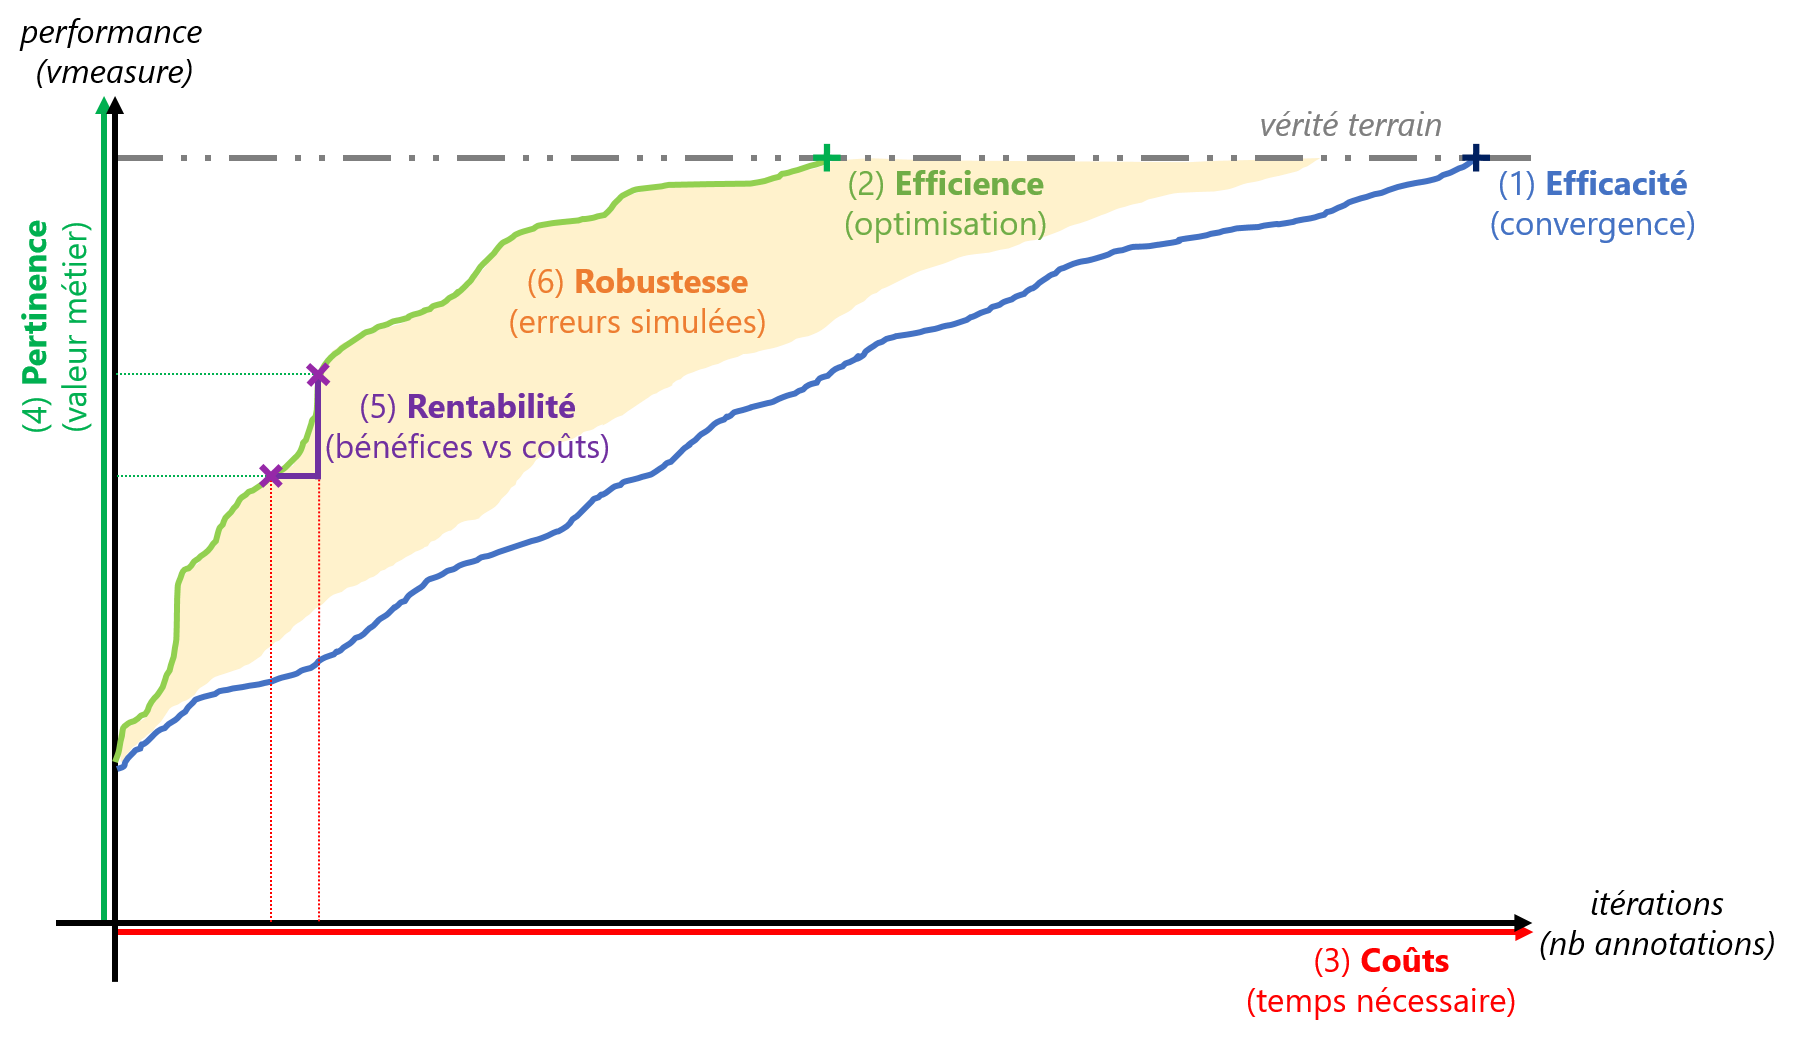
\includegraphics[width=0.8\textwidth]{figures/hypotheses-06-robustesse}
			\caption{Illustration des études réalisées sur le \textit{clustering} interactif (\textit{étape 6/6}) en schématisant l'évolution de la performance (\textit{accord avec la vérité terrain calculé en v-measure}) d'une base d'apprentissage en cours de construction en fonction du nombre d'itérations de la méthode (\textit{nombre d'annotations par un expert métier}).}
			\label{figure:4.6-HYPOTHESE-ROBUSTESSE}
		\end{figure}

	\end{tcolorbox}
	
	%%%
	%%% Subsection 4.6.1: Étude de simulation d'erreurs d'annotations
	%%%
	\subsection{Étude de simulation d'erreurs d'annotations}
	
		%%% Protocole expérimental.
		\subsubsection{Protocole expérimental}
			\todo[inline]{Description succincte du protocole expérimental dans l'encadré d'hypothèse ?}

		%%% Résultats
		\subsubsection{Résultats obtenus}

		%%% Discussion
		\subsubsection{Discussion}
	
	%%%
	%%% Subsection 4.6.2: Étude d'annotation avec des paradigmes différents
	%%%
	\subsection{Étude d'annotation avec des paradigmes différents}
	
		%%% Protocole expérimental.
		\subsubsection{Protocole expérimental}
			\todo[inline]{Description succincte du protocole expérimental dans l'encadré d'hypothèse ?}

		%%% Résultats
		\subsubsection{Résultats obtenus}

		%%% Discussion
		\subsubsection{Discussion}